\chapter{Geometric Simulation}

\begin{figure}
\centering
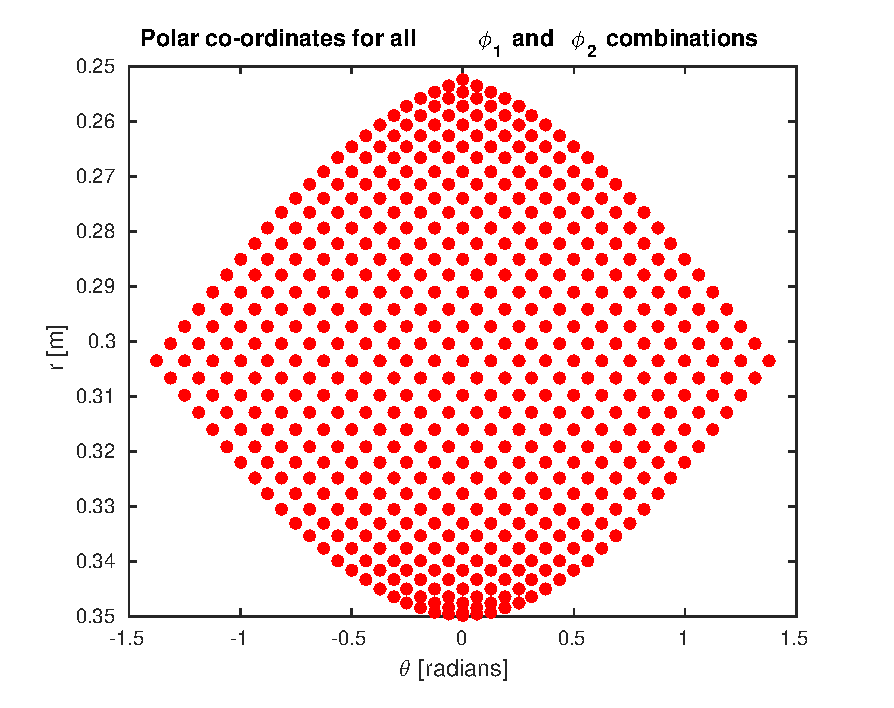
\includegraphics[width=1\textwidth]{images/geometry/forward-kinematic-leg-positions-5-30.eps}
\caption{Polar co-ordinates generated for all $\phi_1$ and $\phi_2$ combinations using forward kinematics: $l_1 = 5cm\ l_2 = 30cm$.}
\label{fig:Polar co-ordinates generated 5-30}
\end{figure}

\begin{figure}
\centering
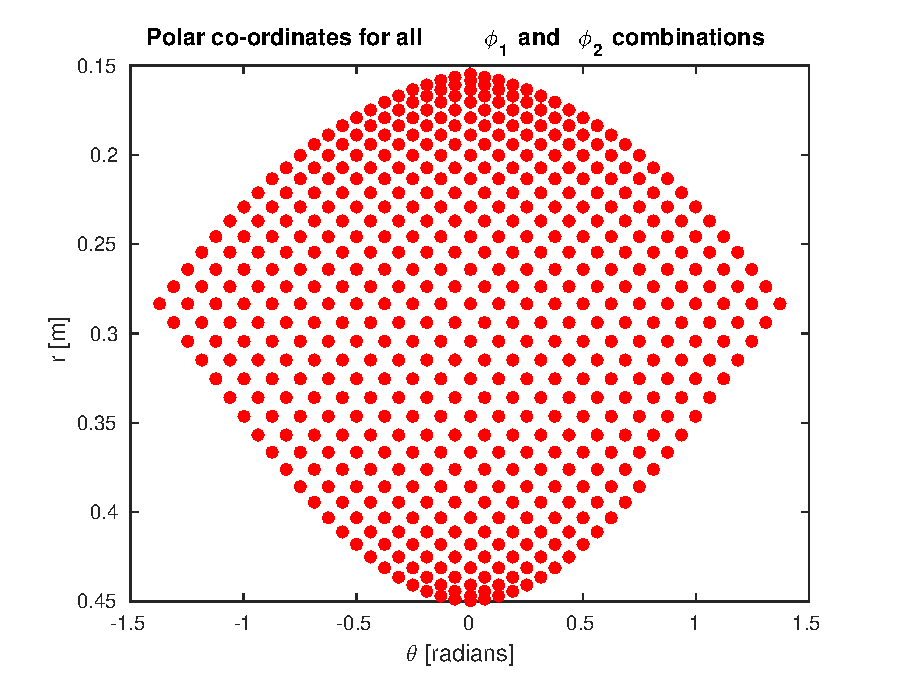
\includegraphics[width=1\textwidth]{images/geometry/forward-kinematic-leg-positions.eps}
\caption{Polar co-ordinates generated for all $\phi_1$ and $\phi_2$ combinations using forward kinematics: $l_1 = 15cm\ l_2 = 30cm$.}
\label{fig:Polar co-ordinates generated 15-30}
\end{figure}

\begin{figure}
\centering
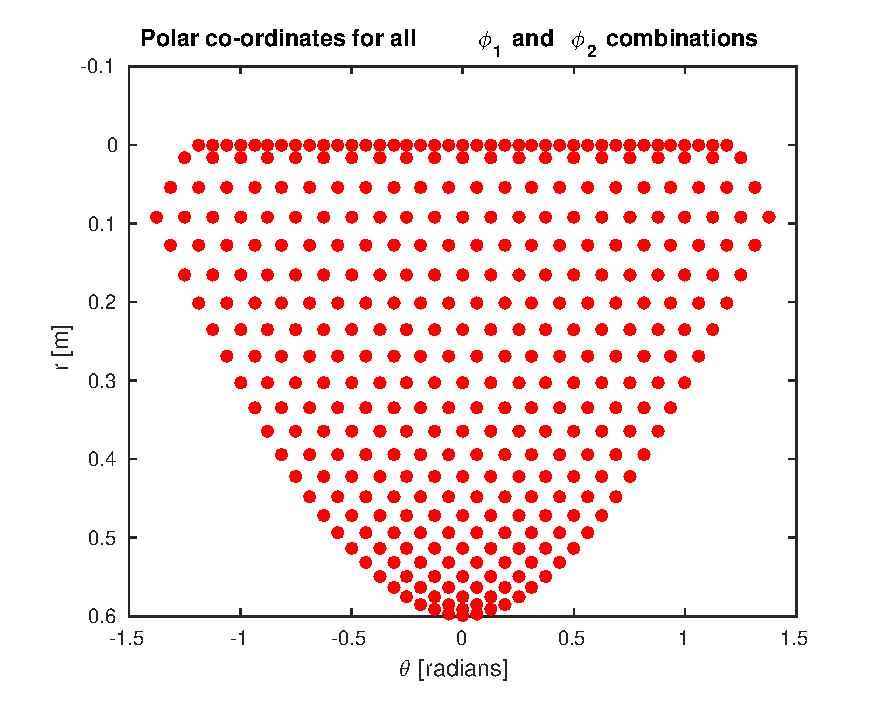
\includegraphics[width=1\textwidth]{images/geometry/forward-kinematic-leg-positions-30-30.eps}
\caption{Polar co-ordinates generated for all $\phi_1$ and $\phi_2$ combinations using forward kinematics: $l_1 = 30cm\ l_2 = 30cm$.}
\label{fig:Polar co-ordinates generated 30-30}
\end{figure}

\begin{figure}
\centering
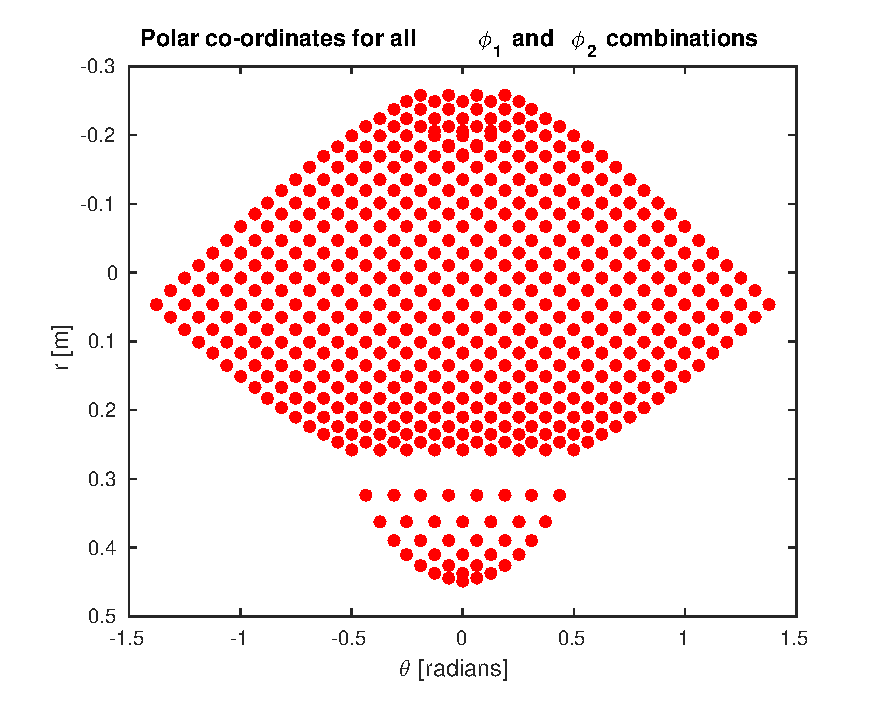
\includegraphics[width=1\textwidth]{images/geometry/forward-kinematic-leg-positions-30-15-complex.eps}
\caption{Polar co-ordinates generated for all $\phi_1$ and $\phi_2$ combinations using forward kinematics: $l_1 = 30cm\ l_2 = 15cm$.}
\label{fig:Polar co-ordinates generated 30-15}
\end{figure}